
%(BEGIN_QUESTION)
% Copyright 2015, Tony R. Kuphaldt, released under the Creative Commons Attribution License (v 1.0)
% This means you may do almost anything with this work of mine, so long as you give me proper credit

\noindent

\vskip 5pt



\vskip 5pt
\begin{center}
\textbf{HMI -- Nivå 1 }
\vskip 5pt 
\textbf{Arbidsoppdrag på egen PC}
\vskip 5pt 
\textbf{HPHMI}
\end{center}

\vskip 10pt 
\textbf{Introdusjon}
\vskip 5pt 
I dette arbeisoppdraget skal du lage en HMI etter prinsippene for HPHMI (High Performance HMI).

\vskip 5pt 
Du skal gjenskapes (ikke kopiere) prosjektet \href{https://rfka-my.sharepoint.com/:u:/g/personal/fred-olav_mosdal_skole_rogfk_no/EbxoQUSK9jxFkJX9XfhvLoMBomsgt_JP02XtAeb4RRNFrA?e=ZfVSqa}{Intro til HPHMI codesys prsjekt}
\vskip 5pt 

\vskip 5pt 

%$$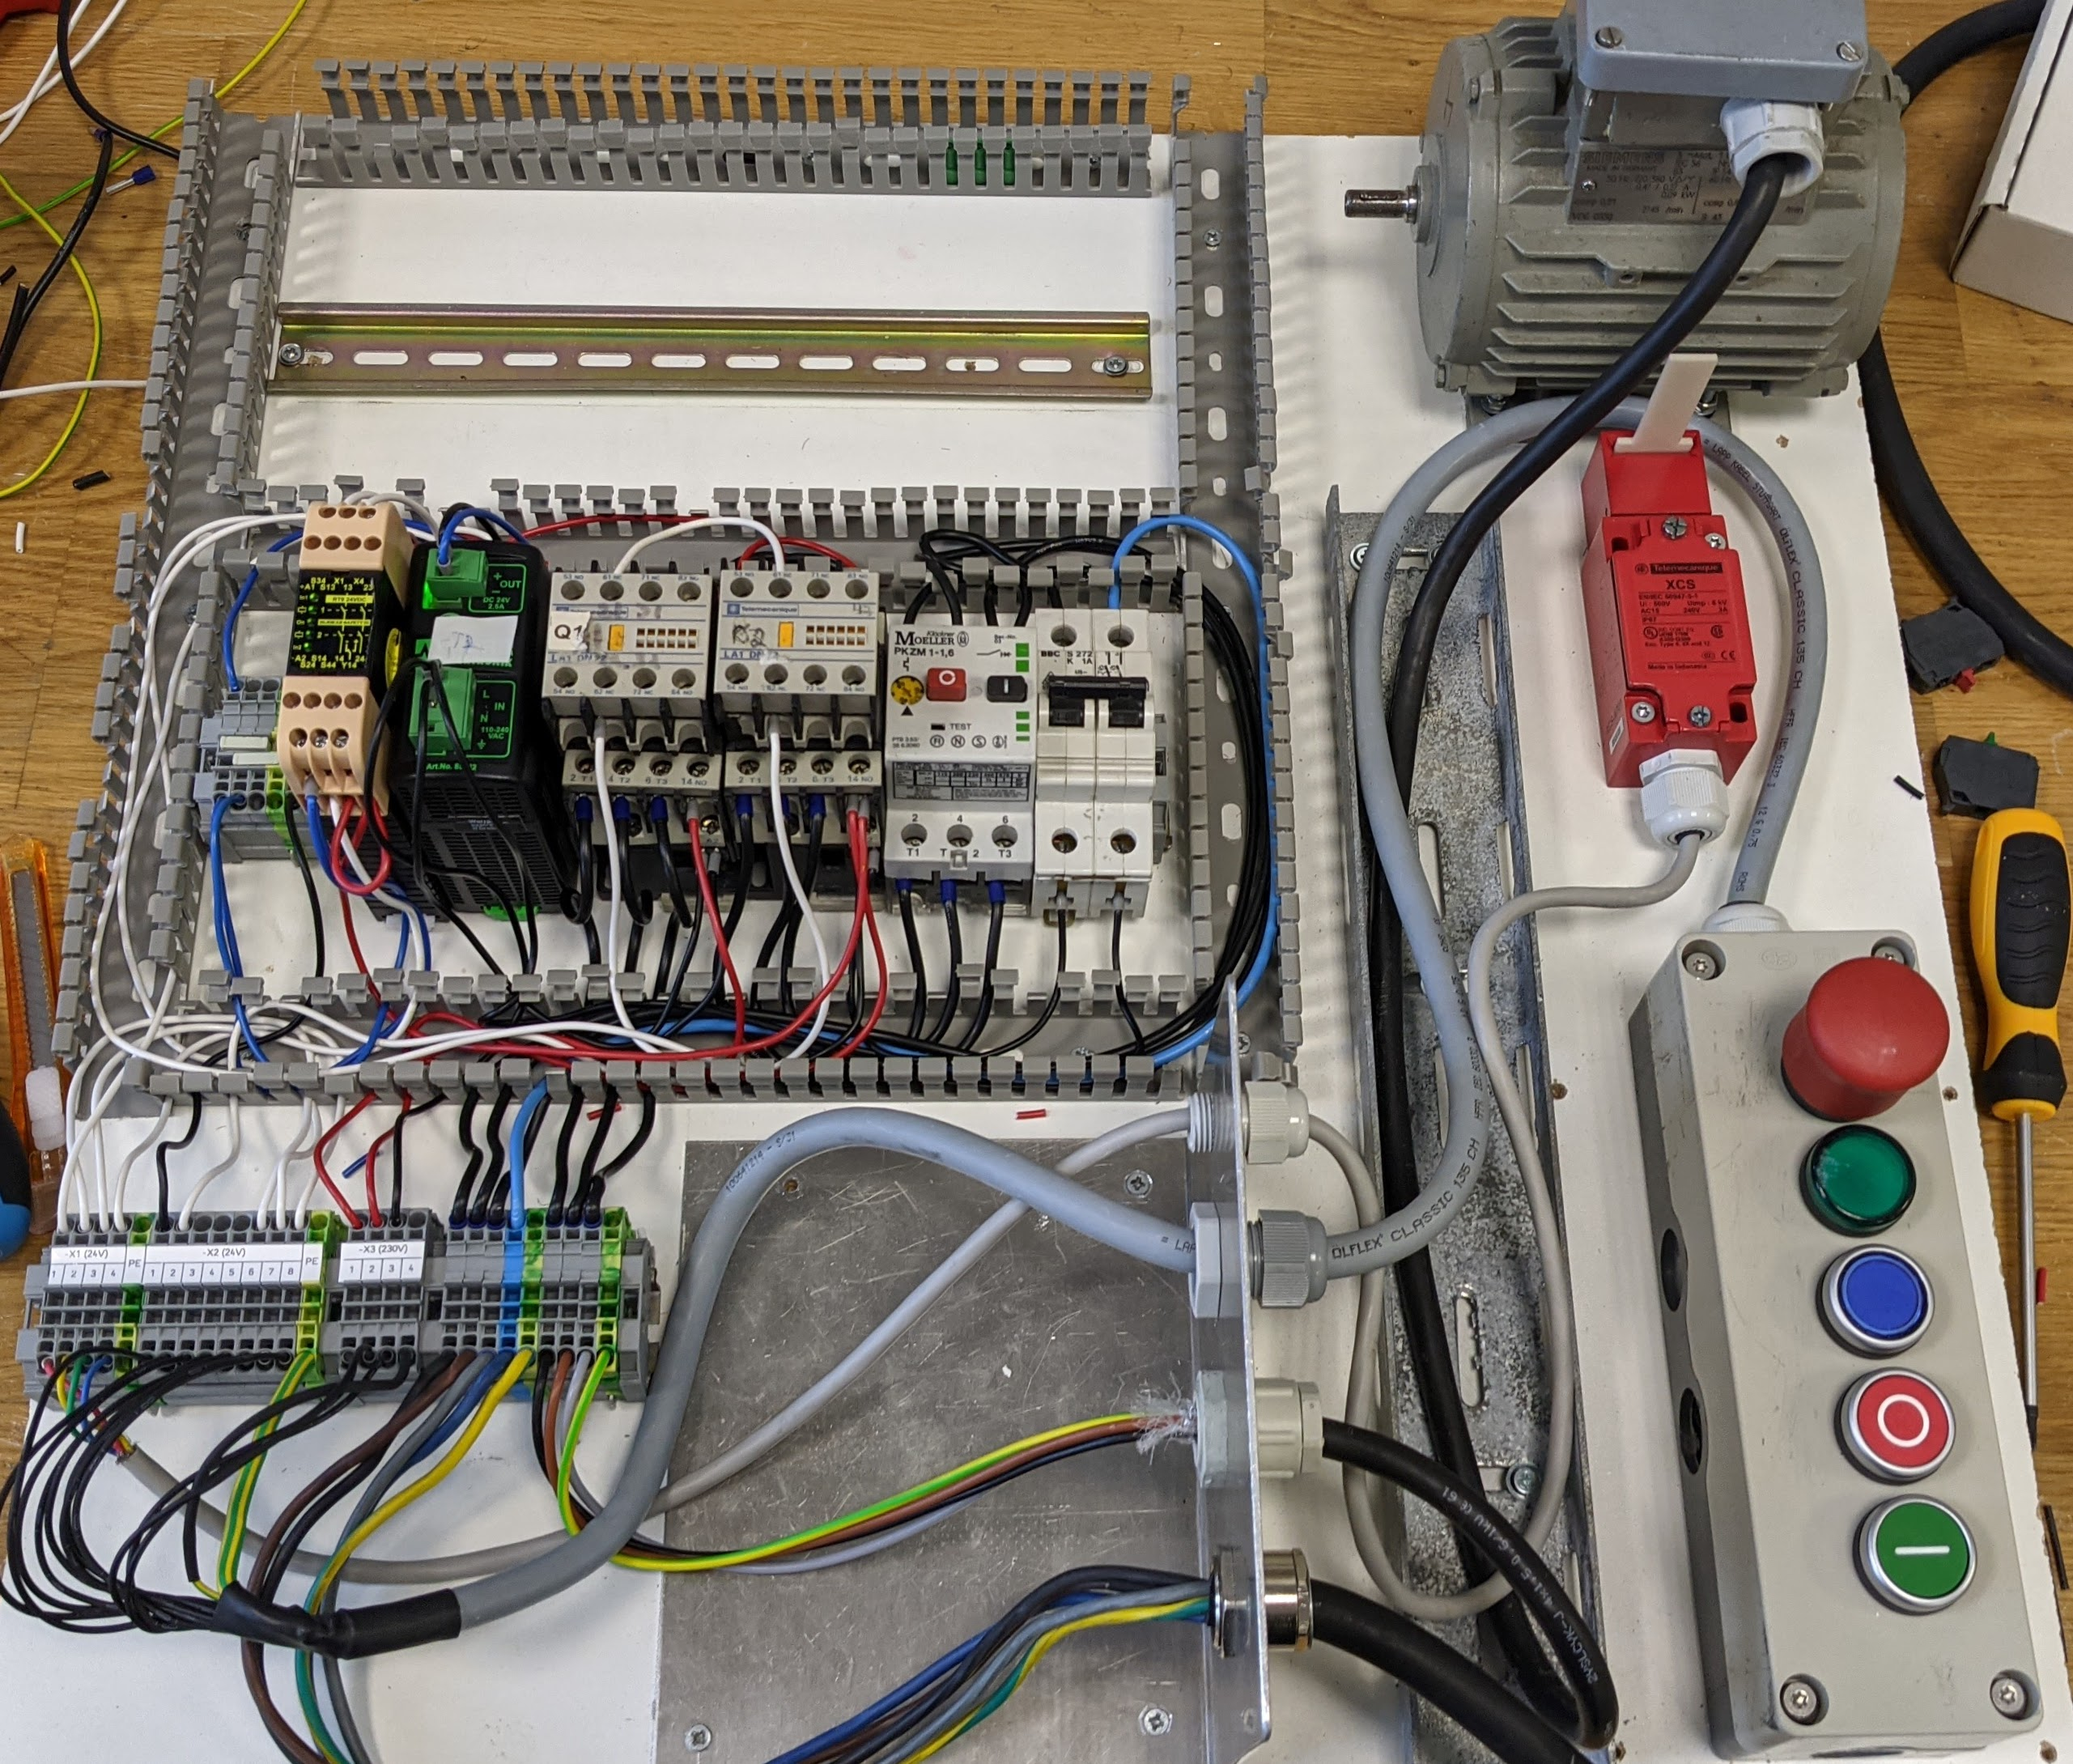
\includegraphics[width=13cm]{i04821x01.jpg}$$\\

\vskip 10pt 
\textbf{Teorioppgaver}

\vskip 5pt 
\href{https://rfka-my.sharepoint.com/:b:/g/personal/fred-olav_mosdal_skole_rogfk_no/EbDgASyqKH5Ni0i6BCYnE04BaRvhWzEjRBcZw8CqgX0Mfw?e=e0zKzU}{Leseoppgave}
\vskip 10pt 
\textbf{Planlegging}


\vskip 10pt 
\textbf{Gjennomføring}

\vskip 10pt 
\textbf{Dokumentasjon}

Beskriv hvordan du planlegger, gjennomfører og dokumenterer denne jobben. 
















\underbar{file i04829}
\vfil \eject
%(END_QUESTION)





%(BEGIN_ANSWER)


%(END_ANSWER)





%(BEGIN_NOTES)


%INDEX% Arbeisdoppdrag, HMI, Nivå 1, Stasjon Egen PC, HPHMI intro

%(END_NOTES)


